Modules mentioned above are defined respecting the signature of some predefined abstract module. For example, the module showed in Figure~\ref{fig:om} is a \om{} based on an abstract module that receives a configuration and returns a neighborhood. In that sense, an example of a concrete \om{} (or just \om{} for simplification sake) can be a function receiving a configuration, and returns a neighborhood composed of $N$ configurations only differing from one value to the input configuration.

In this stage an \as{} is coded through \posl{}. It takes abstract modules as {\it parameters} and combines them with operators. Through the abstract solver, we can also decide what information to be sent to other solvers, by using some operators to send the result of a computation module (see below). Following we present a formal and more detailed presentation of \posl{}'s operators specification. 


The \as{} is the solver's backbone. It joins the \oms{} and the \opchs{} coherently. It is independent from the \oms{} and \opchs{} used in the solver. It means they can be changed or modified during the execution, without altering the general algorithm, but still respecting the main structure. \modified{Each time we combine some of them using \posl's operators, we are creating a \cm. Following we define formally the concept of \textit{module} and \cm.}

\begin{definition}
	\label{def:module}
We call {\bf module} to (and it is denoted by the letter $\mathcal{M}$):
\begin{enumerate}\renewcommand{\labelitemi}{\scriptsize$\blacksquare$}
\item A \om{} or
\item A \opch{} or
\item $\left[\mathcal{M}_1 \text{ OP } \mathcal{M}_2\right]$: The composition of two modules $\mathcal{M}_1$ and $\mathcal{M}_2$ to be executed sequentially, one after the other, and returning an output depending on the nature of the operator \emph{OP}; or\label{subdef:seq}
\item $\lbk\mathcal{M}_1 \text{ OP } \mathcal{M}_2\rbk$: The composition of two modules $\mathcal{M}_1$ and $\mathcal{M}_2$ to be executed and returning an output depending on the nature of the operator \emph{OP}. These two modules will be executed in parallel if and only if \emph{OP} supports parallelism, (i.e. some modules will be executed sequentially although they were grouped this way); or sequentially otherwise.\label{subdef:par}
\end{enumerate}
We denote the space of the modules by $\mathbb{M}$.
We call \cms{} to the composition of modules described in \ref{subdef:seq} and \ref{subdef:par}.
\end{definition}

Following we will define some operators included in \posl{} framework. In order to group modules, like in Definition \ref{def:module}(\ref{subdef:seq}) and \ref{def:module}(\ref{subdef:par}), we will use $\left|.\right|$ as generic grouper.

%$M\textcircled{p}t$

%\begin{example}
%Suppose that we have the following \module s for selecting a configuration from a defined set (neighborhood): {\sc SelectRandom} selects a random configuration $S^*$ from $\mathcal{V}(S)$, and {\sc SelectBest} selects the $S^*=\argmax\left\{f\left(S_i\right)\right\}, \forall S_i \in\mathcal{V}(S)$. Then, we can define a \module $\mathcal{M}$ that selects the best configuration in the neighborhood, but sometimes it takes a random one:
%\mybox{
%	$\mathcal{M}_1 \leftarrow$ {\sc SelectRandom}\\
%	$\mathcal{M}_2 \leftarrow$ {\sc SelectBest}\\
%	$\mathcal{M} \leftarrow \mathcal{M}_1\circled{$\rho$}\mathcal{M}_2$ 
%}
%\end{example}

%The following operator allows us to execute two modules sequentially one after the other. 

\begin{definition}\label{op:seqexec}
{\bf (Operator Sequential Execution)} Let the modules 
\begin{enumerate}%\begin{inparaenum}[i)]
	\item $\mathcal{M}_1 : \mathcal{D}_1 \rightarrow \mathcal{I}_1$ and 
	\item $\mathcal{M}_2 : \mathcal{D}_2 \rightarrow \mathcal{I}_2$, 
\end{enumerate}%\end{inparaenum} 
be, where $\mathcal{I}_1 \subseteq \mathcal{D}_2$. Then, the operation $\left|\mathcal{M}_1\circled{$\mapsto$} \mathcal{M}_2\right|$ defines the \cm{} $\mathcal{M}_{seq}$ as result of the execution of $\mathcal{M}_1$ followed by $\mathcal{M}_2$:

\[
\mathcal{M}_{seq}:\mathcal{D}_1 \rightarrow \mathcal{I}_2
\]
\end{definition}

This operator is an example of an operator that does not support the execution of its involved \cms{} in parallel, because the input of the second \cm{} is the output of the first one.

The following operator is useful to execute modules sequentially creating bifurcations, subject to some boolean condition:

\begin{definition}\label{op:conditional}
{\bf (Operator Conditional Execution)} Let the modules 
\begin{enumerate}%\begin{inparaenum}[i)]
	\item $\mathcal{M}_1 : \mathcal{D}_1 \rightarrow \mathcal{I}_1$ and  
	\item $\mathcal{M}_2 : \mathcal{D}_2 \rightarrow \mathcal{I}_2$,
\end{enumerate}%\end{inparaenum} 
be, where $\mathcal{D}_1 \subseteq \mathcal{D}_2$. %and $\mathcal{I}_1 \subset \mathcal{I}_2$. 
Then, the operation $\left|\mathcal{M}_1\circled{?}_{<cond>}\mathcal{M}_2\right|$ defines the \cm{} $\mathcal{M}_{cond}$ as result of the sequential execution of $\mathcal{M}_1$ if $<cond>$ is {\bf true} or $\mathcal{M}_2$ otherwise:

\[
\mathcal{M}_{cond}:\mathcal{D}_1\cap\mathcal{D}_2 \rightarrow \mathcal{I}_1 \cup \mathcal{I}_2 
\]
\end{definition}

We can execute modules sequentially creating also cycles.

\begin{definition}\label{op:cyclic}
{\bf (Operator Cyclic Execution)} Let the module $\mathcal{M} : \mathcal{D} \rightarrow \mathcal{I}$ be, where $\mathcal{I} \subseteq \mathcal{D}$. Then, the operation $\left|\circlearrowleft_{<cond>}\mathcal{M}\right|$ defines the \cm{} $\mathcal{M}_{cyc}$ as result of the sequential execution of $\mathcal{M}$ repeated while $<cond>$ remains {\bf true}:

\[
\mathcal{M}_{cyc}:\mathcal{D} \rightarrow \mathcal{I} 
\]
\end{definition}

%In Figure \ref{fig:ex1} we present a simple example of how combining \m s using \af{} operators introduced above. Algorithm \ref{algo:ex1} shows the corresponding code.
%
%\figalgosbs{
%	\includegraphics[width=\textwidth]{Ex1.eps}
%	\caption{}\label{fig:ex1}
%}{
%	\caption{POSL code for Figure \ref{fig:ex1}}
%	\dontprintsemicolon
%	\SetNoline
%	
%	\While{$<\text{stop\_cond}>$}{		
%		$\left[\mathcal{M}_1 \xmapsto[<cond>]{} \left\{\mathcal{M}_2;\mathcal{M}_3\right\}\right] \longmapsto \mathcal{M}_4$\;			
%	}
%	\label{algo:ex1}
%}
%
%

%\posl{} provides the possibility to give variability to the solvers. Depending on the operator, one or both operand modules is executed, but only the output of one of them is returned by the \cm. %We present these operators in two definitions, grouping those which execute only one \m{} operand (Definition~\ref{def:one}) and those which execute both (Definition~\ref{def:both}).

\begin{definition}\label{op:rho}
{\bf (Operator Random Choice)} Let the modules
\begin{enumerate}%\begin{inparaenum}[i)]
	\item $\mathcal{M}_1 : \mathcal{D}_1 \rightarrow \mathcal{I}_1$ and  
	\item $\mathcal{M}_2 : \mathcal{D}_2 \rightarrow \mathcal{I}_2$,
\end{enumerate}%\end{inparaenum} 
be, where $\mathcal{D}_1 \subset \mathcal{D}_2$, % and $\mathcal{I}_1 \subset \mathcal{I}_2$, 
and a probability $\rho$. Then, the operation $\left|M_1\circled{$\rho$}\mathcal{M}_2\right|$ defines the \cm{} $\mathcal{M}_{rho}$ that executes and returns the output of $\mathcal{M}_1$ following the probability $\rho$, or executes and returns the output of $\mathcal{M}_2$ following $(1-\rho)$:

\[
\mathcal{M}_{rho}:\mathcal{D}_1\cap\mathcal{D}_2 \rightarrow \mathcal{I}_1 \cup \mathcal{I}_2 
\]
\end{definition}

The following operator is very useful if the user needs to use a \opch{} into an \as{}. As we explained before, if a \opch{} does not receive any information from other solver, it returns {\it NULL}. This may cause the undesired termination of the solver if we do not pay attention correctly. Next, we introduce the operator \textbf{Operator Not {\it NULL} Execution} and we propose an example to illustrate how to use it in practice.

\begin{definition}\label{op:or}
{\bf (Operator Not {\it NULL} Execution)} Let the modules
\begin{enumerate}%\begin{inparaenum}[i)]
	\item $\mathcal{M}_1 : \mathcal{D}_1 \rightarrow \mathcal{I}_1$ and  
	\item $\mathcal{M}_2 : \mathcal{D}_2 \rightarrow \mathcal{I}_2$,
\end{enumerate}%\end{inparaenum} 
be, where $\mathcal{D}_1 \subseteq \mathcal{D}_2$. % and $\mathcal{I}_1 \subset \mathcal{I}_2$. 
Then, the operation $\left|\mathcal{M}_1\circled{$\vee$}\mathcal{M}_2\right|$ defines the \cm{} $\mathcal{M}_{non}$ that executes $\mathcal{M}_1$ and returns its output if it is not {\it NULL}, or executes $\mathcal{M}_2$ and returns its output otherwise:

\[
\mathcal{M}_{non}:\mathcal{D}_1\cap\mathcal{D}_2 \rightarrow \mathcal{I}_1 \cup \mathcal{I}_2 
\]
\end{definition}

Figure~\ref{fig:2difBeh} shows how to combine a connection module with the \om{} \verb!S! through the operator $\circled{$\vee$}$. Here, the computation module \verb!S! will be executed as long as the \opch{} remains \textit{NULL}, i.e., there is no information coming from outside. This behavior is represented in Figure~\ref{subfig:beh1} by orange lines. If some data has been received through the connection module, it is executed instead of the module \verb!S!, represented in Figure~\ref{subfig:beh2} by blue lines.

\begin{figure}[h]
\centering
\subfloat[][The solver executes the computation module {\bf S} if no information is received through the connection module]{
	\label{subfig:beh1}
	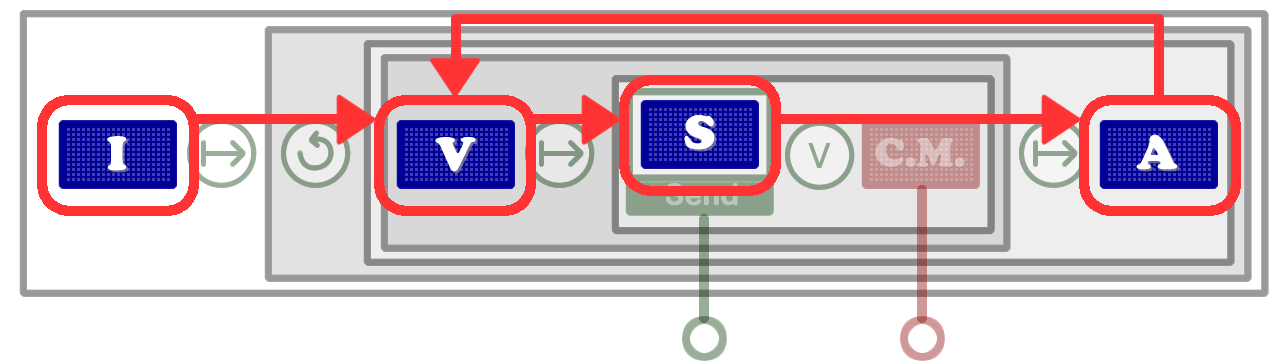
\includegraphics[width=0.7\linewidth]{muta1_v1.png} %[width=0.2\textwidth]{muta1}
}\\
%\hspace{0.05\textwidth}%
\subfloat[][The solver uses the information coming from an external solver]{%
	\label{subfig:beh2}
	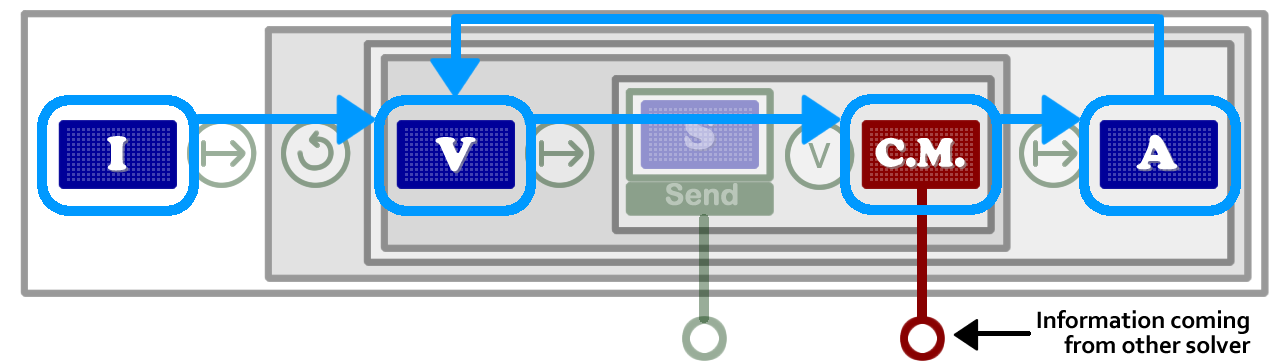
\includegraphics[width=0.7\linewidth]{muta2_v1.png}%[width=0.2\textwidth]{muta2}
}
\caption[]{Two different behaviors in the same solver}
\label{fig:2difBeh}
\end{figure}

\modified{This operator is {\it short-circuit}. It means that if the first argument (module) does not return {\it NULL}, the second will not be executed. \posl{} provides another operator the same functionality but not {\it short-circuit}:}

\begin{definition}\label{op:and}
{\bf (Operator {\it BOTH} Execution)} Let the modules
\begin{enumerate}%\begin{inparaenum}[i)]
	\item $\mathcal{M}_1 : \mathcal{D}_1 \rightarrow \mathcal{I}_1$ and  
	\item $\mathcal{M}_2 : \mathcal{D}_2 \rightarrow \mathcal{I}_2$,
\end{enumerate}%\end{inparaenum} 
be, where $\mathcal{D}_1 \subseteq \mathcal{D}_2$. % and $\mathcal{I}_1 \subset \mathcal{I}_2$. 
Then, the operation $\left|\mathcal{M}_1\circled{$\wedge$}\mathcal{M}_2\right|$ defines the \cm{} $\mathcal{M}_{both}$ that executes both $\mathcal{M}_1$ and $\mathcal{M}_2$, then returns the output of $\mathcal{M}_1$ if it is not {\it NULL}, or the output of $\mathcal{M}_2$ otherwise:

\[
\mathcal{M}_{both}:\mathcal{D}_1\cap\mathcal{D}_2 \rightarrow \mathcal{I}_1 \cup \mathcal{I}_2 
\]
\end{definition}

In the following Definitions, the concepts of {\it cooperative parallelism} and {\it competitive parallelism} are implicitly included. We say that cooperative parallelism exists when two or more processes are running separately, they are independent, and the general result will be some combination of the results of all the involved processes (e.g. Definitions~\ref{op:min} and~\ref{op:max}). On the other hand, competitive parallelism arise when the general result is the solution of the first process terminates (e.g. Definition~\ref{op:race}).

\begin{definition}\label{op:min}
{\bf (Operator Minimum)} Let the modules
\begin{enumerate}%\begin{inparaenum}[i)]
	\item $\mathcal{M}_1 : \mathcal{D}_1 \rightarrow \mathcal{I}_1$ and  
	\item $\mathcal{M}_2 : \mathcal{D}_2 \rightarrow \mathcal{I}_2$,
\end{enumerate}%\end{inparaenum} 
be, where $\mathcal{D}_1 \subseteq \mathcal{D}_2$. %and $\mathcal{I}_1 \subset \mathcal{I}_2$. 
Let also $o_1$ and $o_2$ be the outputs of $\mathcal{M}_1$ and $\mathcal{M}_2$ respectively, and assume that there exist some order criteria between them. Then, the operation $\left|\mathcal{M}_1\circled{m}\mathcal{M}_2\right|$ defines the \cm{} $\mathcal{M}_{min}$ that executes $\mathcal{M}_1$ and returns $\min\left\{o_1,o_2\right\}$:

\[
\mathcal{M}_{min}:\mathcal{D}_1\cap\mathcal{D}_2 \rightarrow \mathcal{I}_1 \cup \mathcal{I}_2 
\]
\end{definition}

Similarly we define the operator \textbf{Maximum}:

\begin{definition}\label{op:max}
{\bf (Operator Maximum)} Let the modules
\begin{enumerate}%\begin{inparaenum}[i)]
	\item $\mathcal{M}_1 : \mathcal{D}_1 \rightarrow \mathcal{I}_1$ and  
	\item $\mathcal{M}_2 : \mathcal{D}_2 \rightarrow \mathcal{I}_2$,
\end{enumerate}%\end{inparaenum} 
be, where $\mathcal{D}_1 \subseteq \mathcal{D}_2$. %and $\mathcal{I}_1 \subset \mathcal{I}_2$. 
Let also $o_1$ and $o_2$ be the outputs of $\mathcal{M}_1$ and $\mathcal{M}_2$ respectively, and assume that there exist some order criteria between them. Then, the operation $\left|\mathcal{M}_1\circled{M}\mathcal{M}_2\right|$ defines the \cm{} $\mathcal{M}_{max}$ that executes $\mathcal{M}_1$ and returns $\max\left\{o_1,o_2\right\}$:

\[
\mathcal{M}_{max}:\mathcal{D}_1\cap\mathcal{D}_2 \rightarrow \mathcal{I}_1 \cup \mathcal{I}_2 
\]
\end{definition}

\begin{definition}\label{op:race}
{\bf (Operator Race)} Let the modules
\begin{enumerate}%\begin{inparaenum}[i)]
	\item $\mathcal{M}_1 : \mathcal{D}_1 \rightarrow \mathcal{I}_1$ and  
	\item $\mathcal{M}_2 : \mathcal{D}_2 \rightarrow \mathcal{I}_2$,
\end{enumerate}%\end{inparaenum} 
be, where $\mathcal{D}_1 \subseteq \mathcal{D}_2$ and $\mathcal{I}_1 \subset \mathcal{I}_2$. Then, the operation $\left|\mathcal{M}_1\circled{$\shortdownarrow$}\mathcal{M}_2\right|$ defines the \cm{} $\mathcal{M}_{race}$ that executes both modules $\mathcal{M}_1$ and $\mathcal{M}_2$, and returns the output of the module ending first:

\[
\mathcal{M}_{race}:\mathcal{D}_1\cap\mathcal{D}_2 \rightarrow \mathcal{I}_1 \cup \mathcal{I}_2 
\]
\end{definition}

%
%\figalgosbs{
%	\includegraphics[width=\textwidth]{Ex2.eps}
%	\caption{}\label{fig:ex2}
%}{
%\caption{POSL code for Figure \ref{fig:ex2}}
%\dontprintsemicolon
%\SetNoline	
%	$\mathcal{M}_1 \longmapsto \left[\left[\mathcal{M}_4 \circled{$\shortdownarrow$} \mathcal{M}_5\right]\circled{$\times$}\left[\mathcal{M}_2\longmapsto\mathcal{M}_3\right]\right]$\; 
%	$\longmapsto\mathcal{M}_6$\;			
%\label{algo:ex2}
%}
%
%%\begin{example}
%%Suppose that we have the following \module s for selecting a configuration from a defined set (neighborhood): {\sc SelectRandom} selects a random configuration $S^*$ from $\mathcal{V}(S)$, and {\sc SelectBest} selects the $S^*=\argmax\left\{f\left(S_i\right)\right\}, \forall S_i \in\mathcal{V}(S)$. Then, we can define a \module $\mathcal{M}$ that selects the best configuration in the neighborhood, but sometimes it takes a random one:
%%\mybox{
%%	$\mathcal{M}_1 \leftarrow$ {\sc SelectRandom}\\
%%	$\mathcal{M}_2 \leftarrow$ {\sc SelectBest}\\
%%	$\mathcal{M} \leftarrow \mathcal{M}_1\circled{$\rho$}\mathcal{M}_2$ 
%%}
%%\end{example}


The operators presented in Definitions~\ref{op:min}, \ref{op:max} and~\ref{op:race} are very useful in terms of sharing not only information between solvers, but also {\it behaviors}. If one of the operands is a \opch{} it can receive an external solver's \om{}, providing the opportunity to instantiate it in the current solver. The operator either instantiates that module if it is not null, and executes it; or it executes the other operand module otherwise.

Some others operators can be useful dealing with {\it sets}.

\begin{definition}\label{op:union}
{\bf (Operator Union)} Let the modules
\begin{enumerate}%\begin{inparaenum}[i)]
	\item $\mathcal{M}_1 : \mathcal{D}_1 \rightarrow \mathcal{I}_1$ and  
	\item $\mathcal{M}_2 : \mathcal{D}_2 \rightarrow \mathcal{I}_2$,
\end{enumerate}%\end{inparaenum} 
be, where $\mathcal{D}_1 \subseteq \mathcal{D}_2$. %and $\mathcal{I}_1 \subset \mathcal{I}_2$. 
Let also $V_1$ and $V_2$ be the outputs of $\mathcal{M}_1$ and $\mathcal{M}_2$ respectively. Then, the operation $\left|\mathcal{M}_1\circled{$\cup$}\mathcal{M}_2\right|$ defines the \cm{} $\mathcal{M}_{\cup}$ that executes both modules $\mathcal{M}_1$ and $\mathcal{M}_2$, and returns $V_1\cup V_2$:

\[
\mathcal{M}_{\cup}:\mathcal{D}_1\cap\mathcal{D}_2 \rightarrow \mathcal{I}_1 \cup \mathcal{I}_2
\]
\end{definition}

Similarly we define the operators \textbf{Intersection} and \textbf{Subtraction}:

\begin{definition}\label{op:intersec}
{\bf (Operator Intersection)} Let the modules
\begin{enumerate}%\begin{inparaenum}[i)]
	\item $\mathcal{M}_1 : \mathcal{D}_1 \rightarrow \mathcal{I}_1$ and  
	\item $\mathcal{M}_2 : \mathcal{D}_2 \rightarrow \mathcal{I}_2$,
\end{enumerate}%\end{inparaenum} 
be, where $\mathcal{D}_1 \subseteq \mathcal{D}_2$. % and $\mathcal{I}_1 \subset \mathcal{I}_2$. Let also $V_1$ and $V_2$ be the outputs of $\mathcal{M}_1$ and $\mathcal{M}_2$ respectively. Then, the operation $\left|\mathcal{M}_1\circled{$\cap$}\mathcal{M}_2\right|$ defines the \cm{} $\mathcal{M}_{\cap}$ that executes both modules $\mathcal{M}_1$ and $\mathcal{M}_2$, and returns $V_1\cap V_2$:

\[
\mathcal{M}_{\cap}:\mathcal{D}_1\cap\mathcal{D}_2 \rightarrow \mathcal{I}_1 \cup \mathcal{I}_2
\]
\end{definition}

\begin{definition}\label{op:subst}
{\bf (Operator Subtraction)} Let the modules
\begin{enumerate}%\begin{inparaenum}[i)]
	\item $\mathcal{M}_1 : \mathcal{D}_1 \rightarrow \mathcal{I}_1$ and  
	\item $\mathcal{M}_2 : \mathcal{D}_2 \rightarrow \mathcal{I}_2$,
\end{enumerate}%\end{inparaenum} 
be, where $\mathcal{D}_1 \subseteq \mathcal{D}_2$. % and $\mathcal{I}_1 \subset \mathcal{I}_2$. 
Let also $V_1$ and $V_2$ be the outputs of $\mathcal{M}_1$ and $\mathcal{M}_2$ respectively. Then, the operation $\left|\mathcal{M}_1\circled{-}\mathcal{M}_2\right|$ defines the \cm{} $\mathcal{M}_{-}$ that executes both modules $\mathcal{M}_1$ and $\mathcal{M}_2$, and returns $V_1 - V_2$:

\[
\mathcal{M}_{-}:\mathcal{D}_1\cap\mathcal{D}_2 \rightarrow \mathcal{I}_1 \cup \mathcal{I}_2
\]
\end{definition}

Now, we define the operators that allow us to send information to outside, i.e. other solvers. We can send two types of information: 
\begin{inparaenum}[i)]
	\item we can execute the \om{} and send its output, or 
	\item we can send the \om{} itself.
\end{inparaenum}. This utility is very useful in terms of sharing behaviors between solvers.

\begin{definition}\label{op:osend}
{\bf (Sending Data Operator)} Let the module $\mathcal{M} : \mathcal{D} \rightarrow \mathcal{I}$ be. Then, the operation $\left|\llparenthesis \mathcal{M}\rrparenthesis^{o}\right|$ defines the \cm{} $\mathcal{M}_{sendD}$ that executes the module $\mathcal{M}$ then return and sends its output to outside:

\[
\mathcal{M}_{sendD}:\mathcal{D} \rightarrow \mathcal{I}
\]
\end{definition}

Similarly we define the operator \textbf{Send Module}:

\begin{definition}\label{op:msend}
{\bf (Sending Module Operator)} Let the module $\mathcal{M} : \mathcal{D} \rightarrow \mathcal{I}$ be. Then, the operation $\left|\llparenthesis \mathcal{M}\rrparenthesis^{m}\right|$ defines the \cm{} $\mathcal{M}_{sendM}$ that executes the module $\mathcal{M}$, then returns its output and sends the module itself to outside:

\[
\mathcal{M}_{sendM}:\mathcal{D} \rightarrow \mathcal{I}
\]
\end{definition}


Once all desired abstract modules are linked together with operators, we obtain what we call an \as. To implement a concrete solver from an \as, one must instantiate each abstract module with a concrete one respecting the required signature. From the same \as, one can implement many different concrete solvers simply by instantiating abstract modules with different concrete modules.

An \as{} is defined as follow: after declaring an \mbox{\tet{\bf abstract solver}} and its name, the first line defines the list of signatures of \oms, the second one the list of signatures of \opchs, then the algorithm of the solver is defined is the solver's body, between \mbox{\tet{\bf begin}} and \mbox{\tet{\bf end}}. For instance, Algorithm~\ref{algo:as_example} illustrate the abstract solver corresponding to Figure~\ref{subfig:as}.


\begin{algorithm}[H]
\dontprintsemicolon
\SetNoline
\SetKwProg{myproc}{}{}{}
\myproc{\tet{\bf abstract solver} as\_01\;
\tet{\bf computation} : $I, V, S, A$ \; 
\tet{\bf connection}: $C.M.$}{
	\Begin{
		%\While{$($\Iter $< K_1)$}
		%{
			$I$ \sec \; %\circled{$\mapsto$}$\;
			\While{$($\Iter \% $K_2)$}{
				$V$ \sec $\left[C.M.\textbf{  } \circled{$\vee$} \textbf{  } \llparenthesis S\rrparenthesis^o\right]$ \sec $A$\;
			}
		%}
	}
}
\caption{\posl{} pseudo-code for the \as{} presented in Figure~\ref{subfig:as}}\label{algo:as_example}
\end{algorithm}	